% l = 8

\begin{figure}[h]
\begin{center}
\subfloat{
\resizebox{8cm}{5cm}{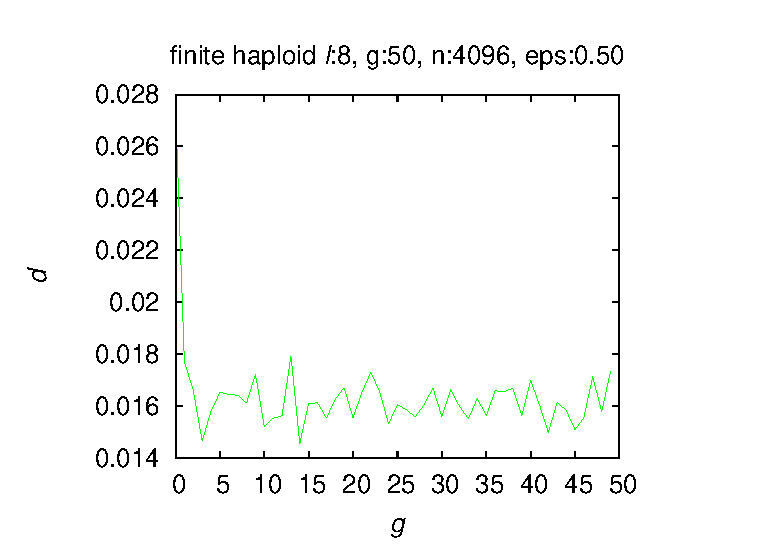
\includegraphics{figures/eps/vio/mu/b8/e0.5/n00004096_fin_hap.eps}}} \hspace{-3em}%
\subfloat{
\resizebox{8cm}{5cm}{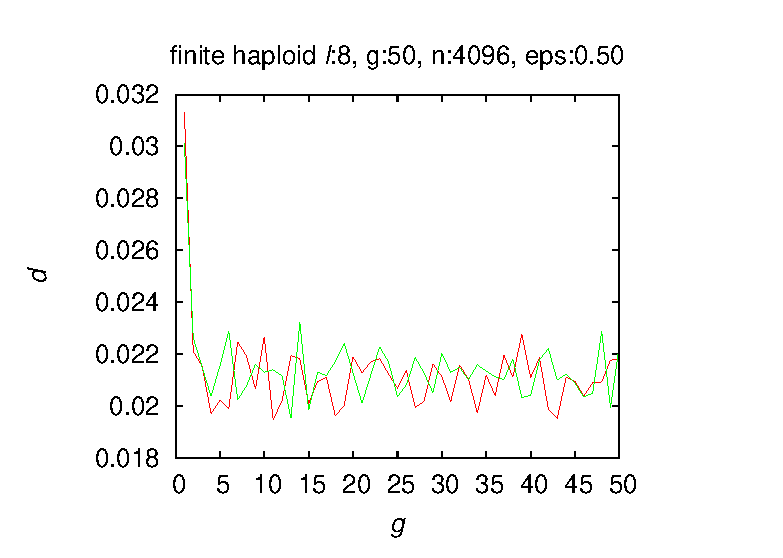
\includegraphics{figures/eps/vio/mu/b8/e0.5/n00004096_fin_hap_wovio.eps}}}\vspace{-1em} \hspace{-3em}%
\end{center}
\begin{center}
\subfloat{
\resizebox{8cm}{5cm}{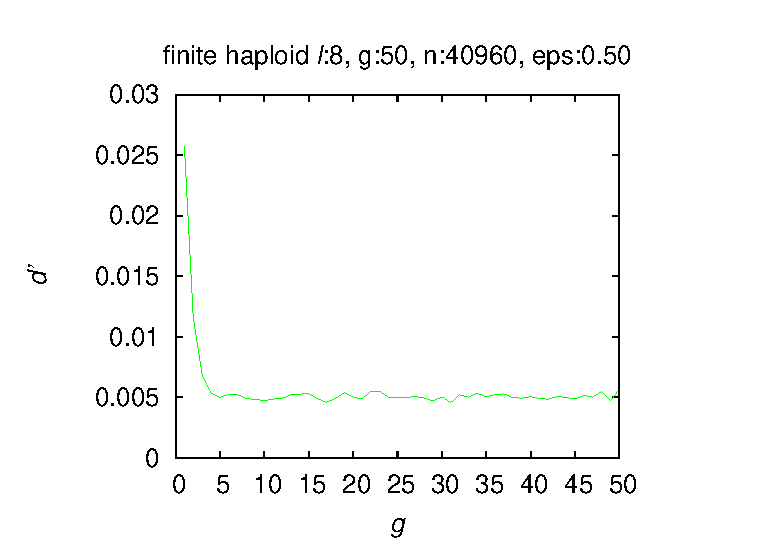
\includegraphics{figures/eps/vio/mu/b8/e0.5/n00040960_fin_hap.eps}}} \hspace{-3em}%
\subfloat{
\resizebox{8cm}{5cm}{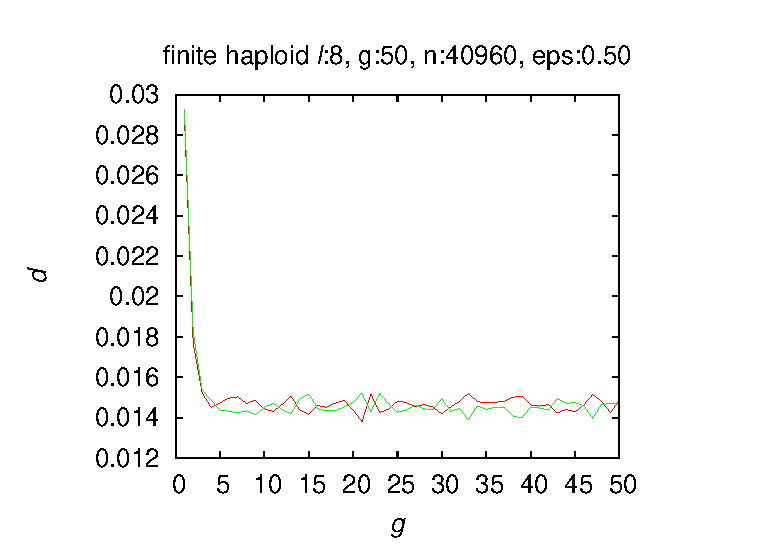
\includegraphics{figures/eps/vio/mu/b8/e0.5/n00040960_fin_hap_wovio.eps}}}\vspace{-1em} \hspace{-3em}%
\end{center}

\begin{center}
\subfloat{
\resizebox{8cm}{5cm}{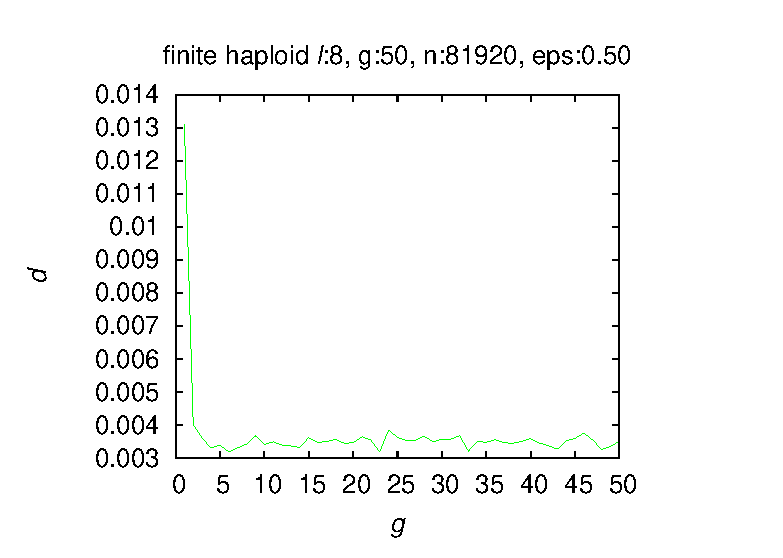
\includegraphics{figures/eps/vio/mu/b8/e0.5/n00081920_fin_hap.eps}}} \hspace{-3em}%
\subfloat{
\resizebox{8cm}{5cm}{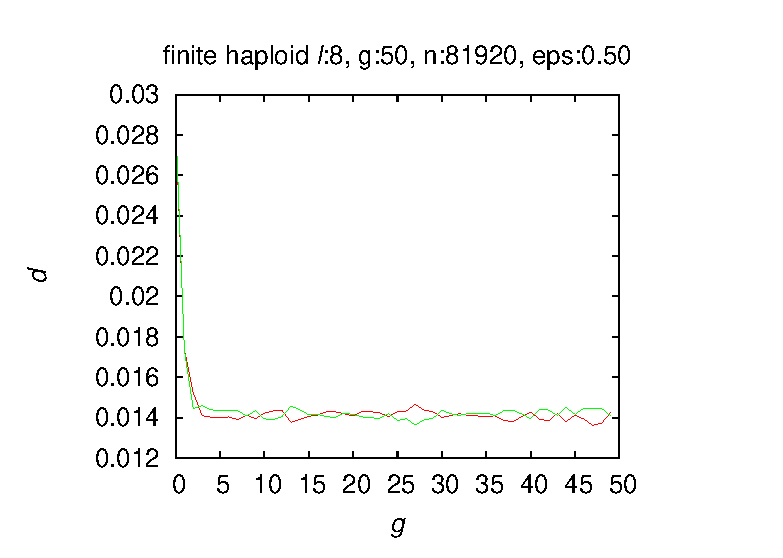
\includegraphics{figures/eps/vio/mu/b8/e0.5/n00081920_fin_hap_wovio.eps}}}\vspace{-1em} \hspace{-3em}%
\end{center}

\begin{center}
\subfloat{
\resizebox{8cm}{5cm}{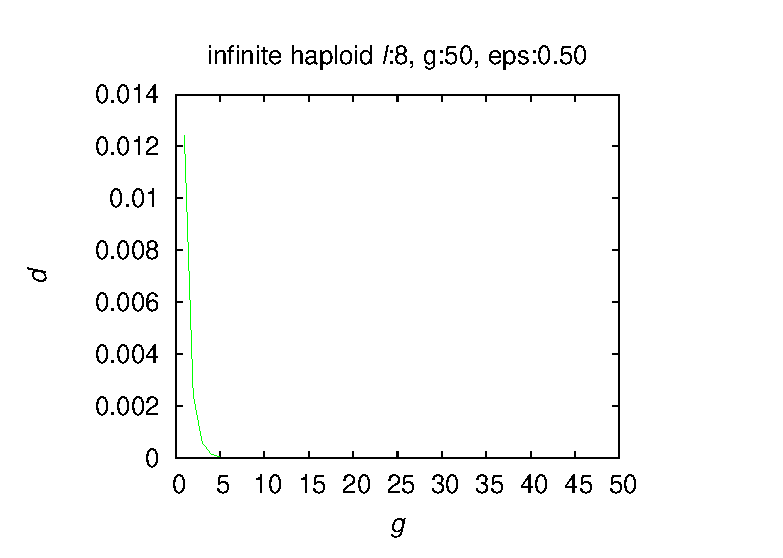
\includegraphics{figures/eps/vio/mu/b8/e0.5/inf_hap.eps}}}\hspace{-3em}%
\subfloat{
\resizebox{8cm}{5cm}{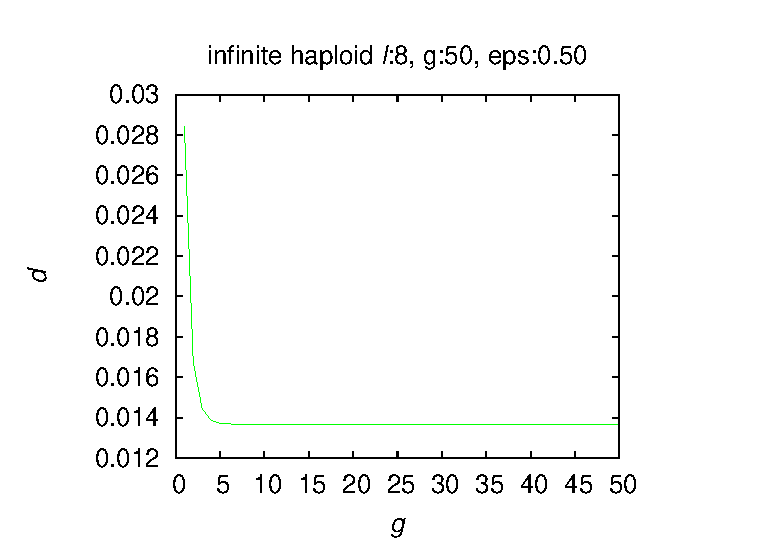
\includegraphics{figures/eps/vio/mu/b8/e0.5/inf_hap_wovio.eps}}}\vspace{-0.5em} \hspace{-3em}%


\caption{\textbf{Infinite and finite haploid population oscillation behavior in case of violation in $\bm{\mu}$ for genome length $\ell = 8$ and $\bm{\epsilon} = 0.5$:} 
  In left column, $d'$ is distance of finite population of size $n$ or infinite population to limit $\bm{z}^\ast$ for $g$ generations. In right column, $d$ is distance of finite population or infinite population to limits $\bm{p}^\ast$ and $\bm{q}^\ast$ without violation.}
\label{oscillation_8h_vio_mu_0.5}
\end{center}
\end{figure}

% l = 10

\begin{figure}[h]
\begin{center}
\subfloat{
\resizebox{8cm}{5cm}{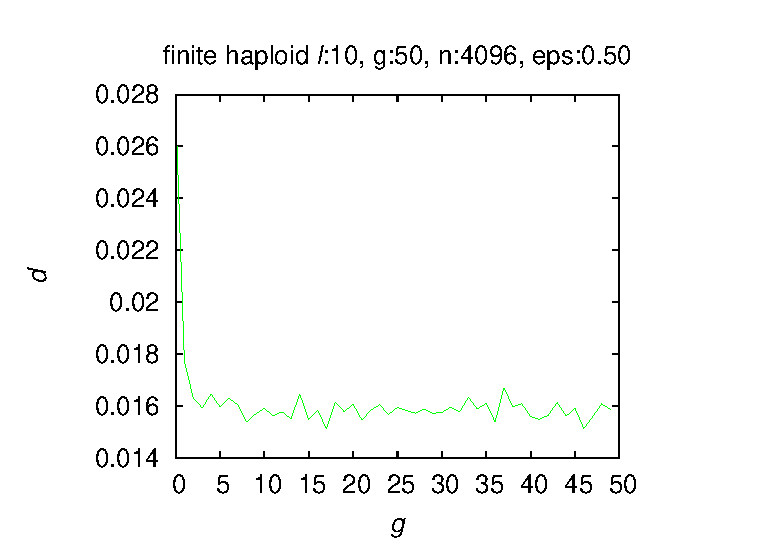
\includegraphics{figures/eps/vio/mu/b10/e0.5/n00004096_fin_hap.eps}}} \hspace{-3em}%
\subfloat{
\resizebox{8cm}{5cm}{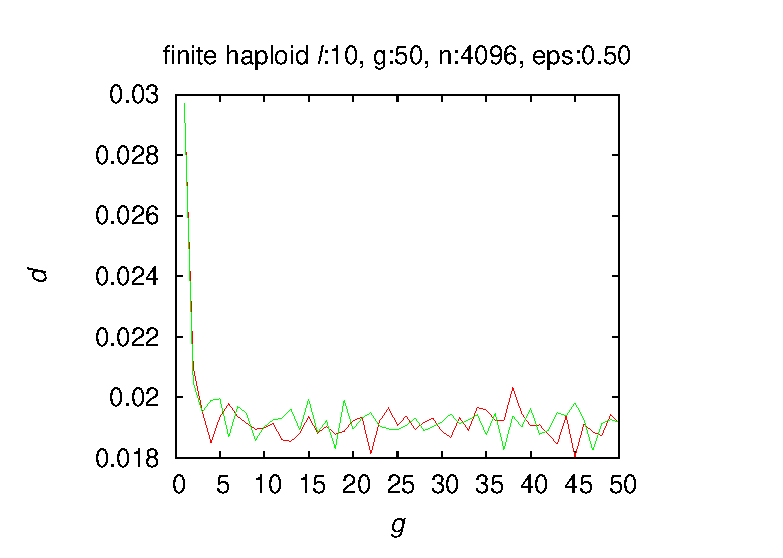
\includegraphics{figures/eps/vio/mu/b10/e0.5/n00004096_fin_hap_wovio.eps}}}\vspace{-1em} \hspace{-3em}%
\end{center}
\begin{center}
\subfloat{
\resizebox{8cm}{5cm}{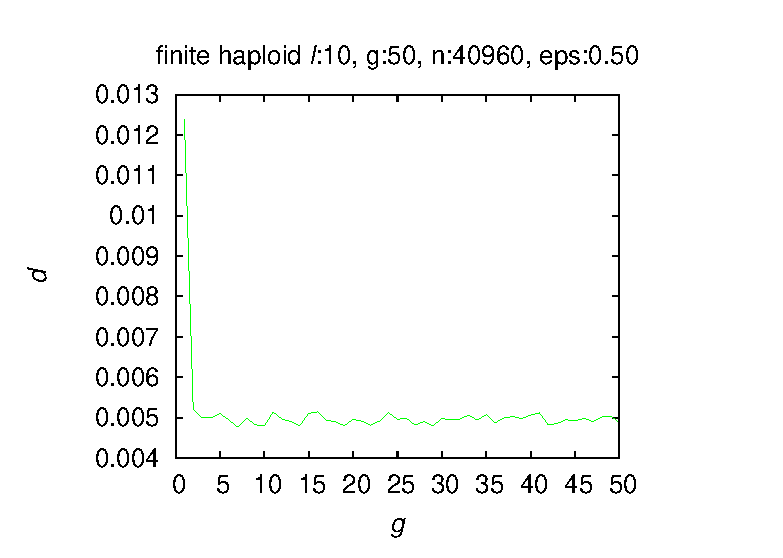
\includegraphics{figures/eps/vio/mu/b10/e0.5/n00040960_fin_hap.eps}}} \hspace{-3em}%
\subfloat{
\resizebox{8cm}{5cm}{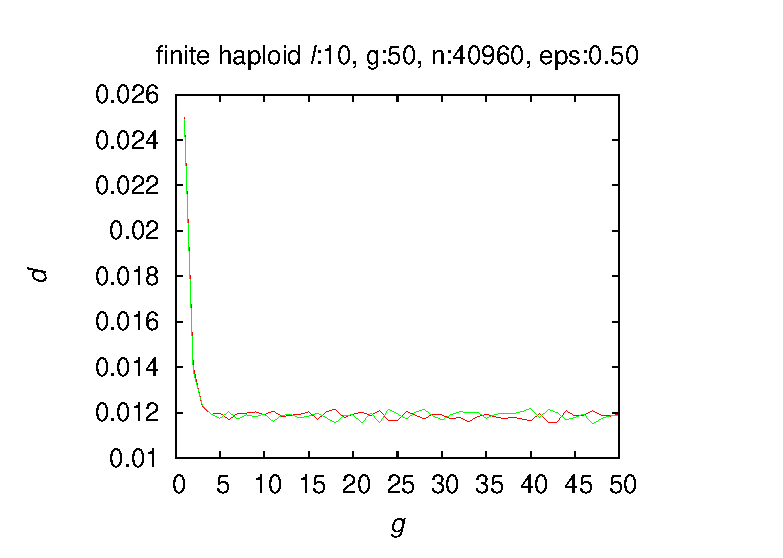
\includegraphics{figures/eps/vio/mu/b10/e0.5/n00040960_fin_hap_wovio.eps}}}\vspace{-1em} \hspace{-3em}%
\end{center}

\begin{center}
\subfloat{
\resizebox{8cm}{5cm}{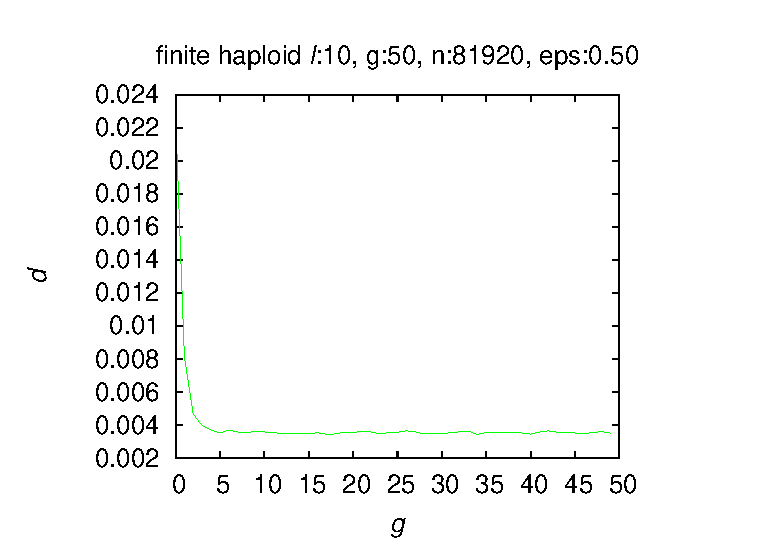
\includegraphics{figures/eps/vio/mu/b10/e0.5/n00081920_fin_hap.eps}}} \hspace{-3em}%
\subfloat{
\resizebox{8cm}{5cm}{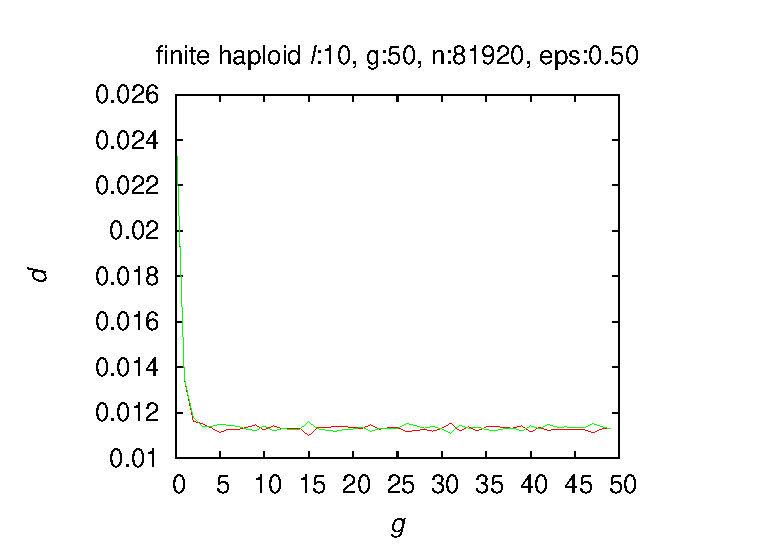
\includegraphics{figures/eps/vio/mu/b10/e0.5/n00081920_fin_hap_wovio.eps}}}\vspace{-1em} \hspace{-3em}%
\end{center}

\begin{center}
\subfloat{
\resizebox{8cm}{5cm}{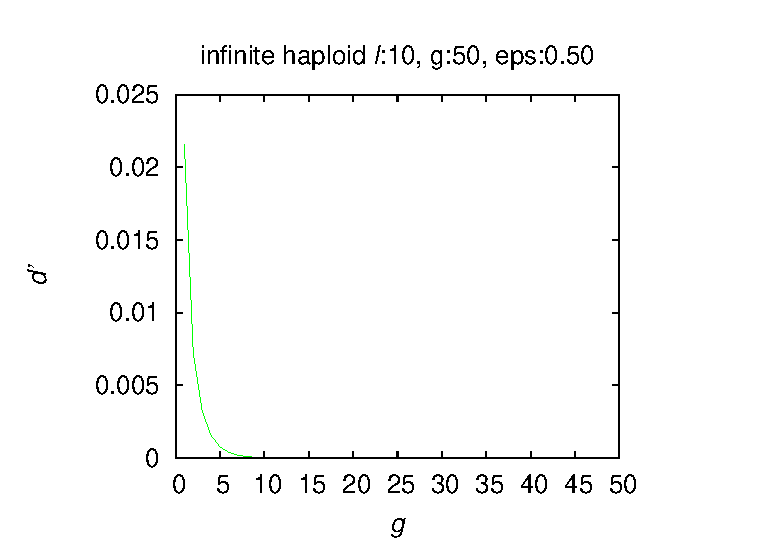
\includegraphics{figures/eps/vio/mu/b10/e0.5/inf_hap.eps}}}\hspace{-3em}%
\subfloat{
\resizebox{8cm}{5cm}{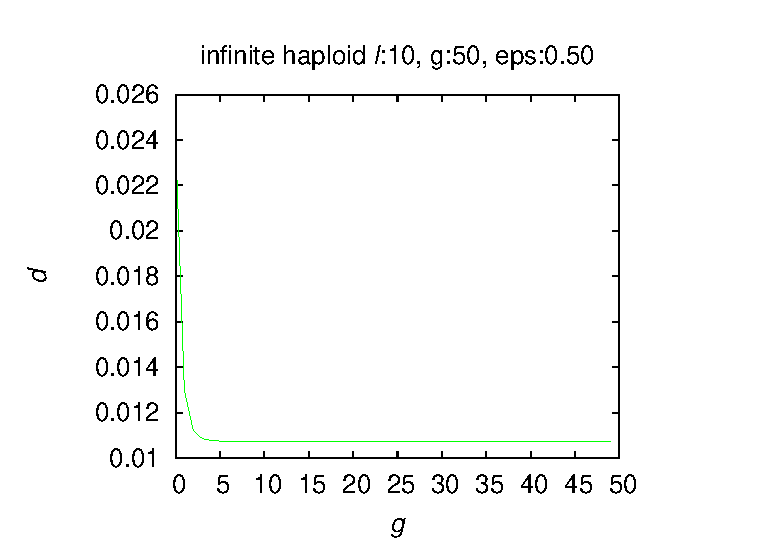
\includegraphics{figures/eps/vio/mu/b10/e0.5/inf_hap_wovio.eps}}}\vspace{-0.5em} \hspace{-3em}%


\caption{\textbf{Infinite and finite haploid population oscillation behavior in case of violation in $\bm{\mu}$ for genome length $\ell = 10$ and $\bm{\epsilon} = 0.5$:} 
  In left column, $d'$ is distance of finite population of size $n$ or infinite population to limit $\bm{z}^\ast$ for $g$ generations. In right column, $d$ is distance of finite population or infinite population to limits $\bm{p}^\ast$ and $\bm{q}^\ast$ without violation.}
\label{oscillation_10h_vio_mu_0.5}
\end{center}
\end{figure}

% l = 12

\begin{figure}[h]
\begin{center}
\subfloat{
\resizebox{8cm}{5cm}{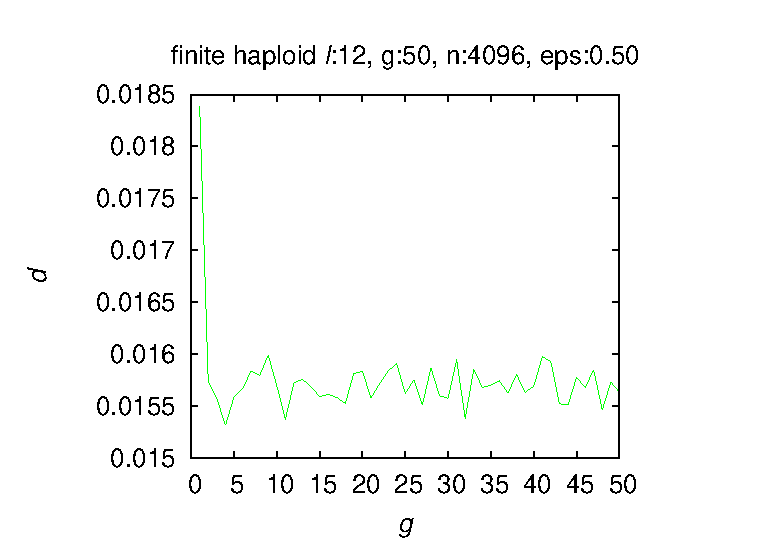
\includegraphics{figures/eps/vio/mu/b12/e0.5/n00004096_fin_hap.eps}}} \hspace{-3em}%
\subfloat{
\resizebox{8cm}{5cm}{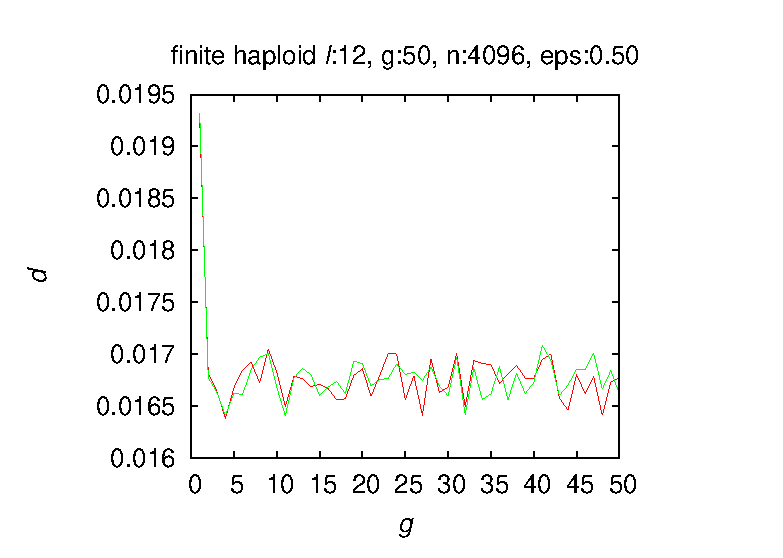
\includegraphics{figures/eps/vio/mu/b12/e0.5/n00004096_fin_hap_wovio.eps}}}\vspace{-1em} \hspace{-3em}%
\end{center}
\begin{center}
\subfloat{
\resizebox{8cm}{5cm}{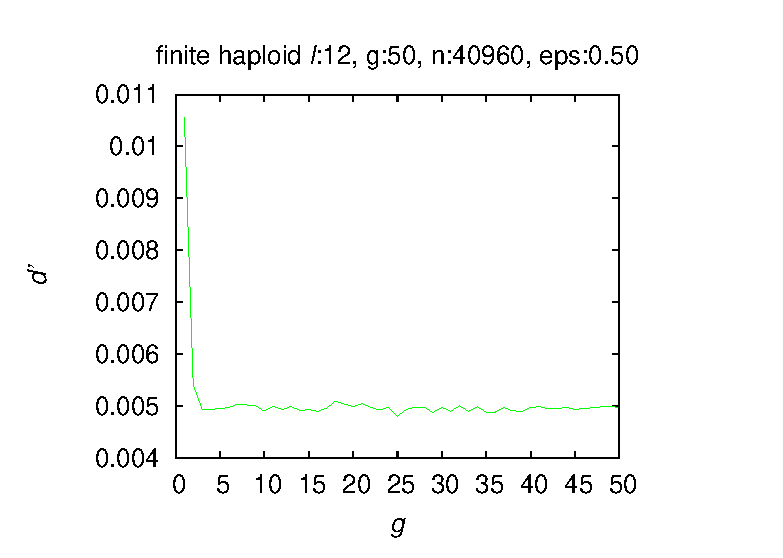
\includegraphics{figures/eps/vio/mu/b12/e0.5/n00040960_fin_hap.eps}}} \hspace{-3em}%
\subfloat{
\resizebox{8cm}{5cm}{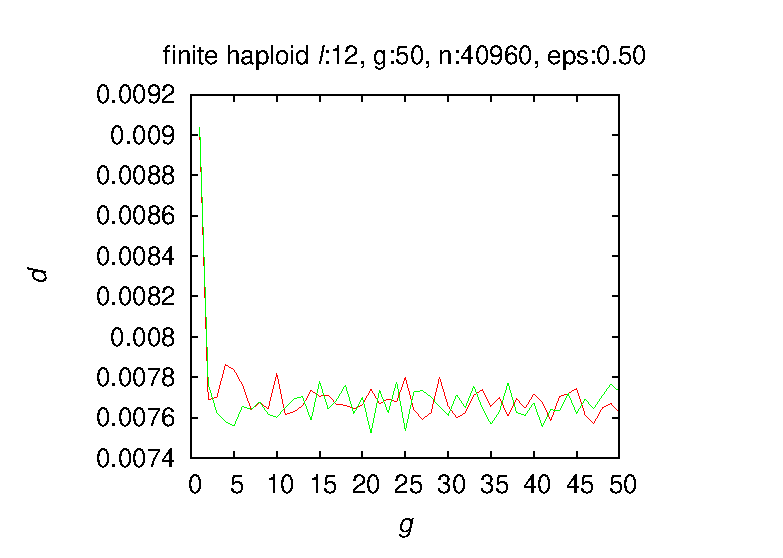
\includegraphics{figures/eps/vio/mu/b12/e0.5/n00040960_fin_hap_wovio.eps}}}\vspace{-1em} \hspace{-3em}%
\end{center}

\begin{center}
\subfloat{
\resizebox{8cm}{5cm}{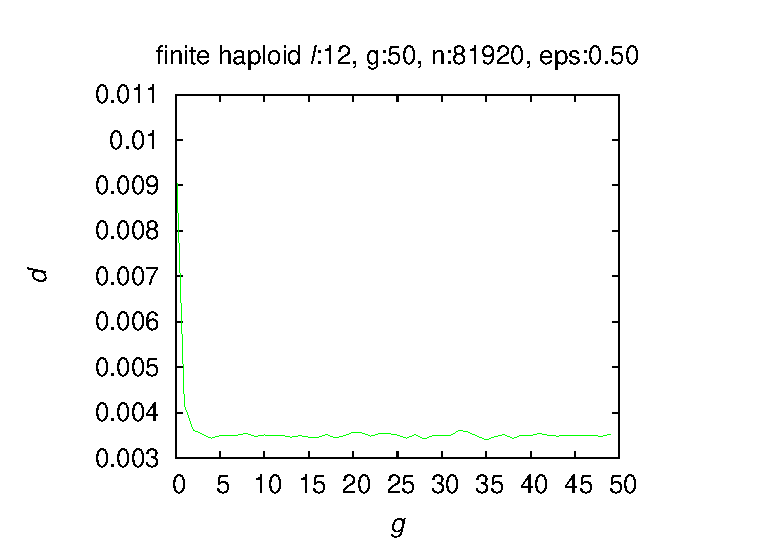
\includegraphics{figures/eps/vio/mu/b12/e0.5/n00081920_fin_hap.eps}}} \hspace{-3em}%
\subfloat{
\resizebox{8cm}{5cm}{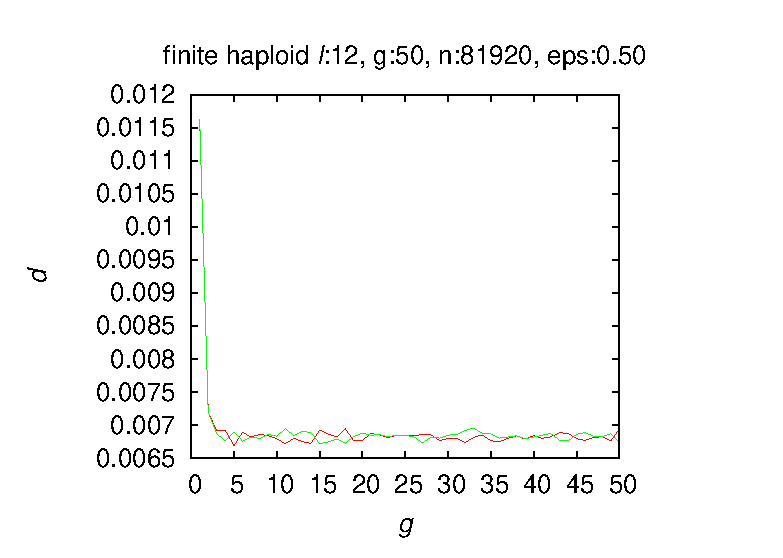
\includegraphics{figures/eps/vio/mu/b12/e0.5/n00081920_fin_hap_wovio.eps}}}\vspace{-1em} \hspace{-3em}%
\end{center}

\begin{center}
\subfloat{
\resizebox{8cm}{5cm}{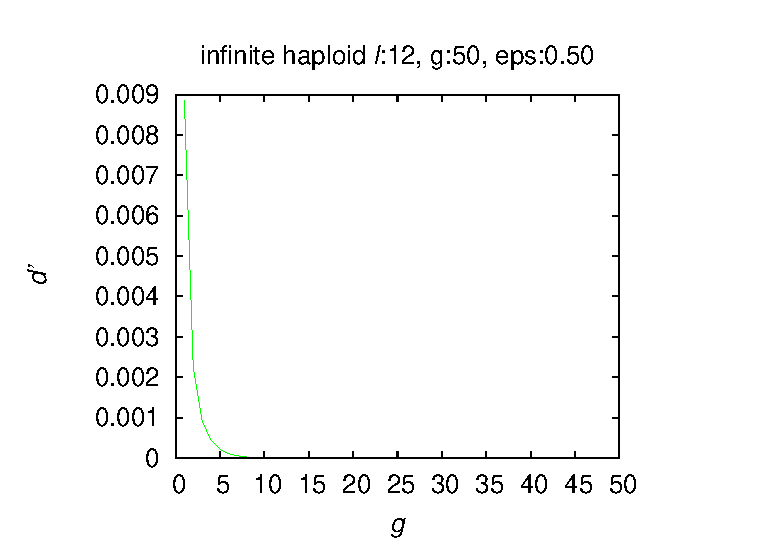
\includegraphics{figures/eps/vio/mu/b12/e0.5/inf_hap.eps}}}\hspace{-3em}%
\subfloat{
\resizebox{8cm}{5cm}{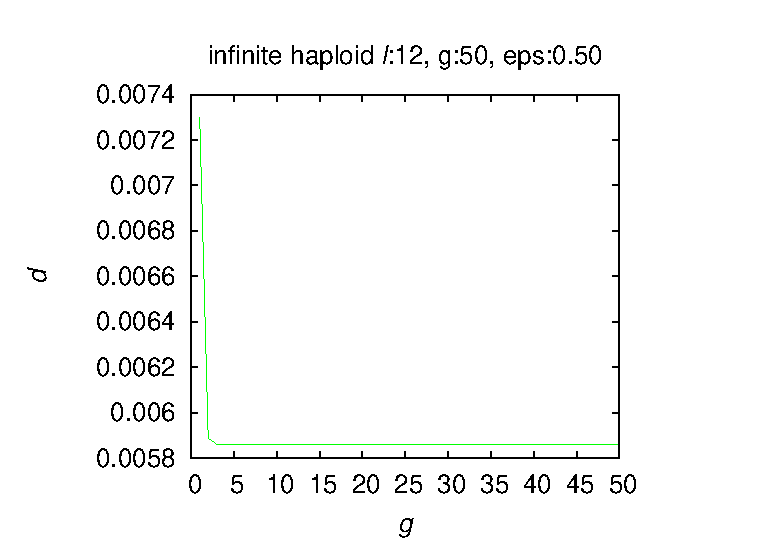
\includegraphics{figures/eps/vio/mu/b12/e0.5/inf_hap_wovio.eps}}}\vspace{-0.5em} \hspace{-3em}%


\caption{\textbf{Infinite and finite haploid population oscillation behavior in case of violation in $\bm{\mu}$ for genome length $\ell = 12$ and $\bm{\epsilon} = 0.5$:} 
  In left column, $d'$ is distance of finite population of size $n$ or infinite population to limit $\bm{z}^\ast$ for $g$ generations. In right column, $d$ is distance of finite population or infinite population to limits $\bm{p}^\ast$ and $\bm{q}^\ast$ without violation.}
\label{oscillation_12h_vio_mu_0.5}
\end{center}
\end{figure}

% l = 14

\begin{figure}[h]
\begin{center}
\subfloat{
\resizebox{8cm}{5cm}{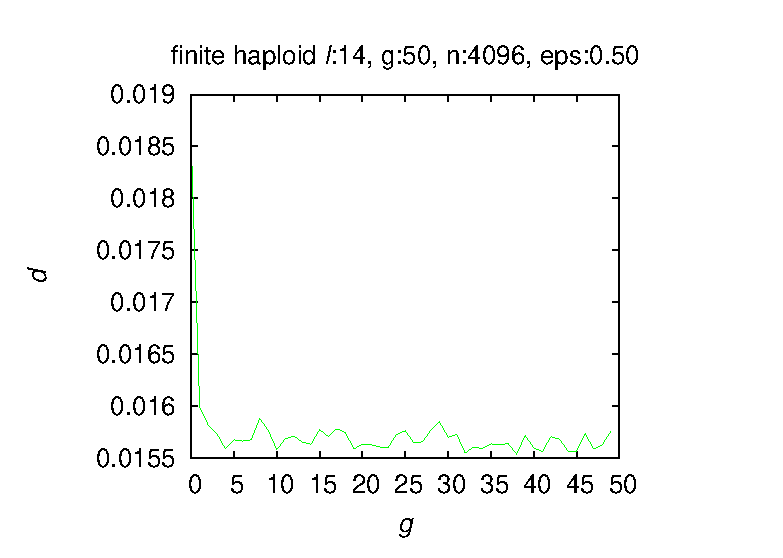
\includegraphics{figures/eps/vio/mu/b14/e0.5/n00004096_fin_hap.eps}}} \hspace{-3em}%
\subfloat{
\resizebox{8cm}{5cm}{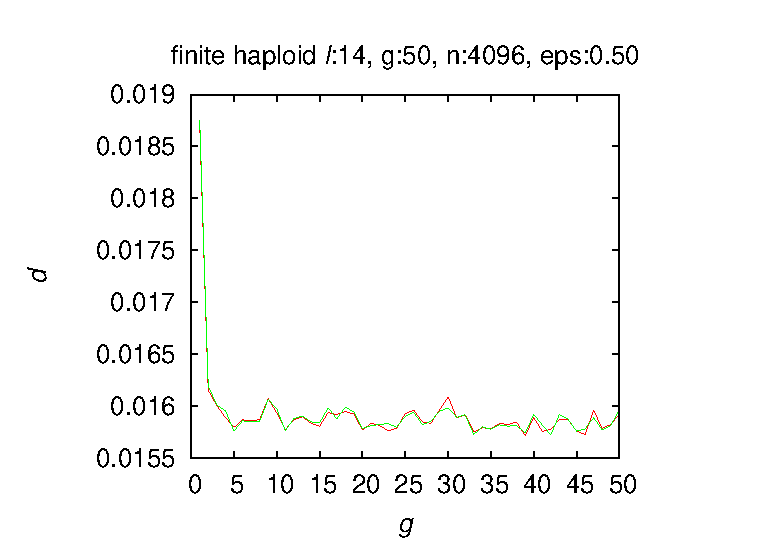
\includegraphics{figures/eps/vio/mu/b14/e0.5/n00004096_fin_hap_wovio.eps}}}\vspace{-1em} \hspace{-3em}%
\end{center}
\begin{center}
\subfloat{
\resizebox{8cm}{5cm}{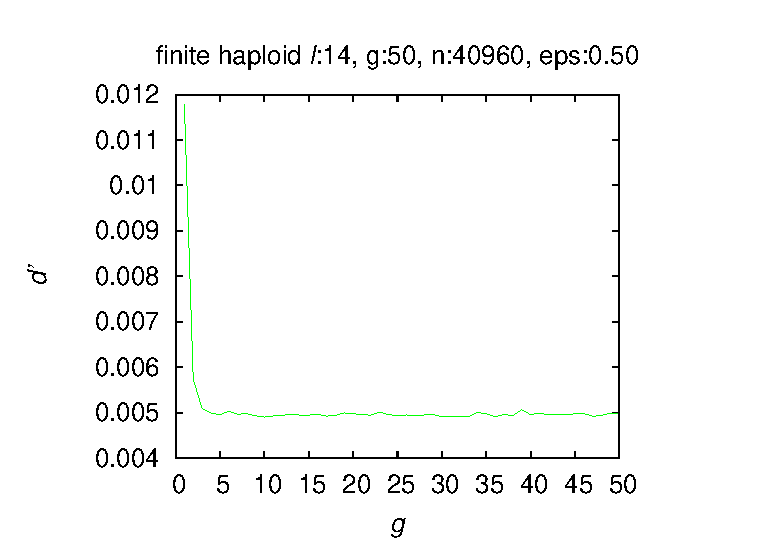
\includegraphics{figures/eps/vio/mu/b14/e0.5/n00040960_fin_hap.eps}}} \hspace{-3em}%
\subfloat{
\resizebox{8cm}{5cm}{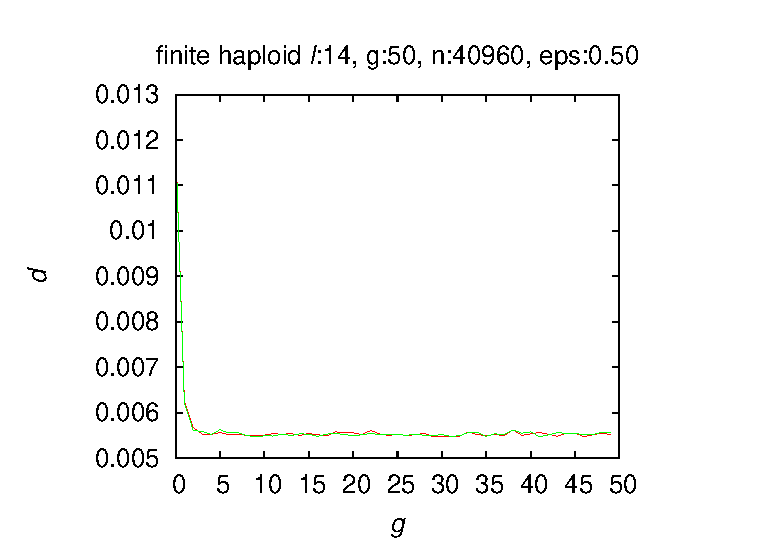
\includegraphics{figures/eps/vio/mu/b14/e0.5/n00040960_fin_hap_wovio.eps}}}\vspace{-1em} \hspace{-3em}%
\end{center}

\begin{center}
\subfloat{
\resizebox{8cm}{5cm}{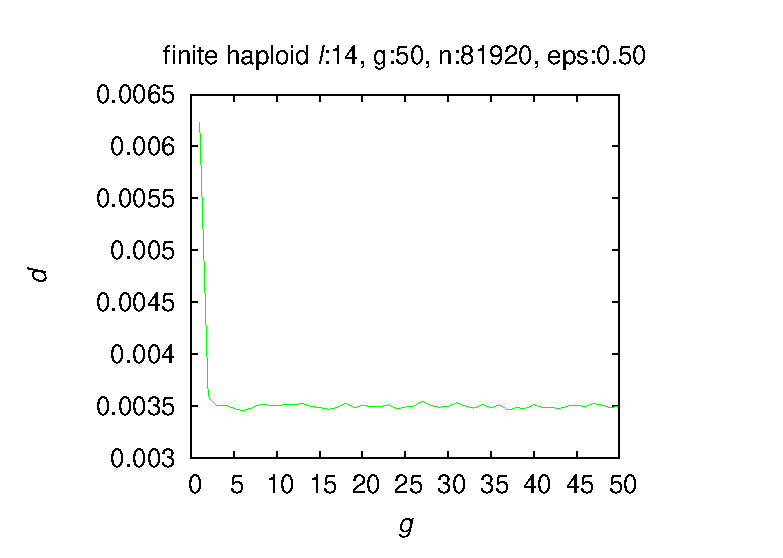
\includegraphics{figures/eps/vio/mu/b14/e0.5/n00081920_fin_hap.eps}}} \hspace{-3em}%
\subfloat{
\resizebox{8cm}{5cm}{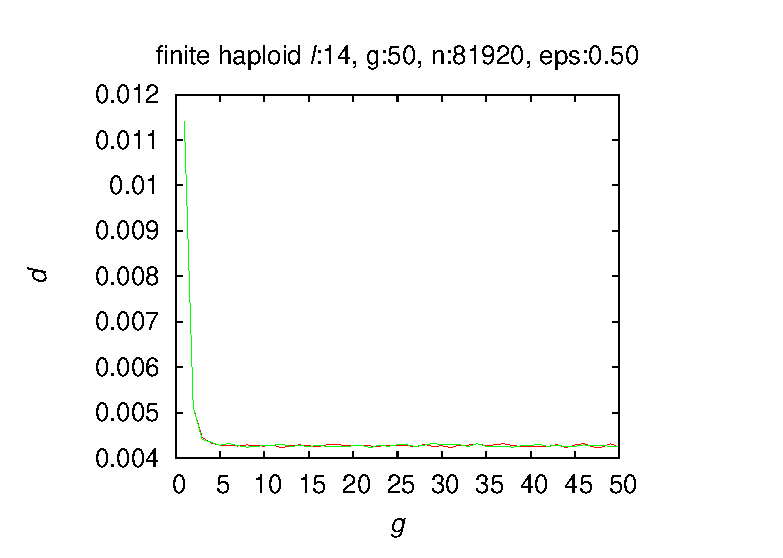
\includegraphics{figures/eps/vio/mu/b14/e0.5/n00081920_fin_hap_wovio.eps}}}\vspace{-1em} \hspace{-3em}%
\end{center}

\begin{center}
\subfloat{
\resizebox{8cm}{5cm}{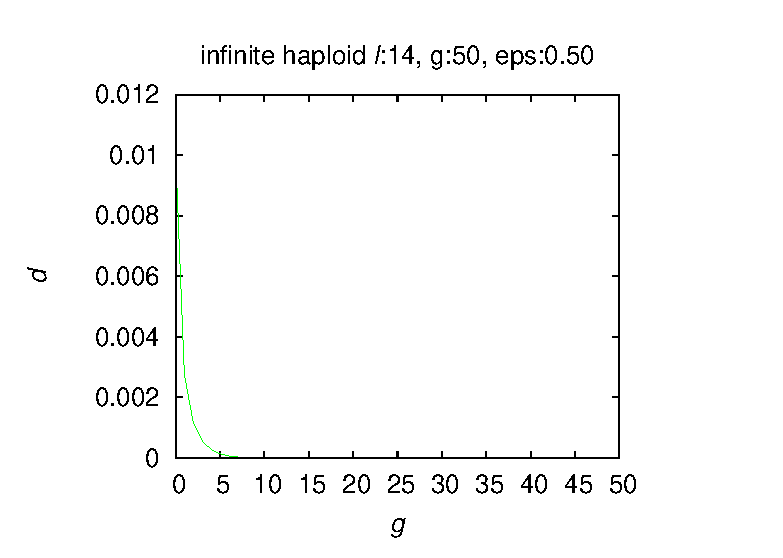
\includegraphics{figures/eps/vio/mu/b14/e0.5/inf_hap.eps}}}\hspace{-3em}%
\subfloat{
\resizebox{8cm}{5cm}{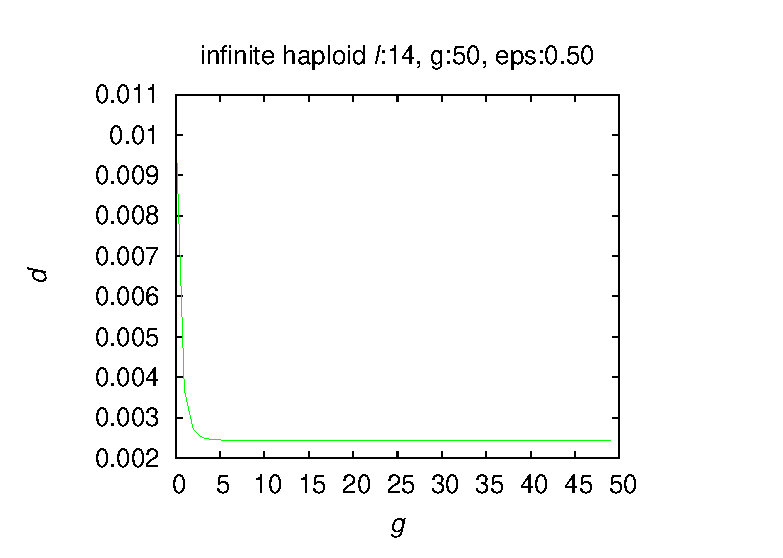
\includegraphics{figures/eps/vio/mu/b14/e0.5/inf_hap_wovio.eps}}}\vspace{-0.5em} \hspace{-3em}%

\caption{\textbf{Infinite and finite haploid population oscillation behavior in case of violation in $\bm{\mu}$ for genome length $\ell = 14$ and $\bm{\epsilon} = 0.5$:} 
  In left column, $d'$ is distance of finite population of size $n$ or infinite population to limit $\bm{z}^\ast$ for $g$ generations. In right column, $d$ is distance of finite population or infinite population to limits $\bm{p}^\ast$ and $\bm{q}^\ast$ without violation.}
\label{oscillation_14h_vio_mu_0.5}
\end{center}
\end{figure}

\clearpage

The right column in figures \ref{oscillation_8h_vio_mu_0.5} through \ref{oscillation_14h_vio_mu_0.5} 
shows distance of finite and infinite haploid populations to non-violation limits $\bm{p^\ast}$ and $\bm{q^\ast}$ with $\bm{\epsilon} \;=\; 0.5$. 
The graphs indicate oscillating behavior of haploid population given violation. 
Neither finite nor infinite populations show noticable oscillation given violation. 
The all zeros mask created in mutation distribution with $\bm{\epsilon} \;=\; 0.5$ has large probability 
of being used during mutation, so oscillation does not occur.

The left column of figures \ref{oscillation_8h_vio_mu_0.5} through \ref{oscillation_14h_vio_mu_0.5} 
shows distance of finite and infinite haploid populations to limit $\bm{z^\ast}$ 
(limit with violation in mutation distribution $\bm{\mu}$) when $\bm{\epsilon} \;=\; 0.5$. 
The distance between finite population and limit $\bm{z}^\ast$ (limit with violation in $\bm{\mu}$ distribution) 
decreases as finite population size increases, 
and finite population shows behavior similar to infinite population behavior as finite population size grows. 
Average distance data for haploid population in case of violation in $\bm{\mu}$ distribution 
with $\bm{\epsilon} \;=\; 0.5$ for different finite population size $N$ are tabulated in table \ref{distanceMuHapEps0.5}.

\begin{table}[ht]
\caption{\textbf{Distance measured for violation in $\bm{\mu}$ with $\bm{\epsilon} \;=\; 0.5$ for haploids:} $\ell$ is genome length, 
average distance between finite and infinite population is tabulated in the last three columns, and last row is expected single step distance.}
\centering
\begin{tabularx}{0.75\textwidth}{ c *{3}{X}}
\toprule
$\ell$ & $N = 4096$ & $N = 40960$ & $N = 81920$ \\
\midrule
8 & 0.0161	&  0.0056	& 0.0042 \\
10 & 0.0161	&  0.0055	& 0.0040 \\
12 & 0.0157	&  0.0051	& 0.0036 \\
14 & 0.0157	&  0.0051	& 0.0036 \\
\midrule
$1/\sqrt{N}$ & 0.0156 & 0.0049 & 0.0035 \\
\bottomrule
\end{tabularx}
\label{distanceMuHapEps0.5}
\end{table}
 
The results in Table \ref{distanceMuHapEps0.5} show average distance 
between finite population and limit $\bm{z^\ast}$ approach expected single step distance 
between finite and infinite population. The distance decreased as $1/\sqrt{N}$. 
Also, the distance decreased as genome length $\ell$ increased for all sizes of finite haploid populations 
with $\bm{\epsilon} \;=\; 0.5$.